\documentclass[xcolor=dvipsnames,10pt,aspectratio=169]{beamer}
%\usetheme[hideallsubsections]{Hannover}
\usetheme[width=1.9cm]{Hannover} % plenty of themes to pick from
\usefonttheme[onlymath]{serif}
\graphicspath{{../../images/}}
\usepackage[utf8]{inputenc}
\usepackage[T1]{fontenc}
\usepackage{amsmath}
\usepackage{amsfonts}
\usepackage{amssymb}
\usepackage{braket}
\usepackage{bm}
\usepackage{textpos}
\usepackage{multicol}
\usepackage{graphicx,hyperref,url}
\usepackage{tikz}
\usepackage{verbatim}
\usepackage{pgfplots}
\usetikzlibrary{arrows,shapes}
\usecolortheme{crane} % plenty of color themes to pick from
\useinnertheme{rectangles}

\definecolor{UBCgreen}{RGB}{30, 77, 43} % UBC Blue (primary)
\definecolor{UBCgold}{RGB}{200, 195, 114} % UBC Grey (secondary)

\setbeamercolor{palette primary}{bg=UBCgreen,fg=white}
\setbeamercolor{palette secondary}{bg=UBCgreen,fg=white}
\setbeamercolor{palette tertiary}{bg=UBCgreen,fg=white}
\setbeamercolor{palette quaternary}{bg=UBCgreen,fg=white}
\setbeamercolor{palette sidebar primary}{fg=black,bg=UBCgold}
\setbeamercolor{palette sidebar secondary}{fg=black,bg=UBCgold}
\setbeamercolor{palette sidebar tertiary}{fg=black,bg=UBCgold}
\setbeamercolor{palette sidebar quaternary}{fg=black,bg=UBCgold}
\setbeamercolor{structure}{fg=UBCgreen} % itemize, enumerate, etc
\setbeamercolor{section in toc}{fg=UBCgreen} % TOC sections
\setbeamercolor{subsection in head/foot}{bg=UBCgold,fg=white}
\setbeamercolor{section in sidebar}{fg=UBCgreen}
\setbeamercolor{section in sidebar}{fg=UBCgreen}
\setbeamerfont{section in sidebar}{size=\small}
\setbeamerfont{title in sidebar}{size=\tiny}
\setbeamerfont{author in sidebar}{size=\tiny}
\setbeamertemplate{page number in head/foot}[appendixframenumber]
\setbeamertemplate{navigation symbols}{\footnotesize\usebeamertemplate{page number in head/foot}}
\setbeamertemplate{frametitle}[default][left,colsep=-4bp,rounded=false]
\setbeamertemplate{section in toc}[bullets]
\addtobeamertemplate{title page}{}{%
    \begin{textblock*}{100mm}(0.445\textwidth,-21.4em)
      
\includegraphics[width=1.5cm]{CSU-Ram-357-617.pdf}
    \end{textblock*}
}
\addtobeamertemplate{frametitle}{}{%
    \begin{textblock*}{100mm}(0.95\textwidth,-0.95cm)
    
\includegraphics[width=0.925cm]{CSU-Ram-357-617.pdf}
    \end{textblock*}
}
\makeatletter
\setbeamertemplate{sidebar canvas \beamer@sidebarside}%
                  [vertical shading][top=UBCgold,bottom=UBCgold]
\makeatother

%\addtobeamertemplate{sidebar left}{}{
%  \hspace{0.3cm}
%  \vspace{0.2cm}
%  
\includegraphics[align = l, width = 1cm]{CSU-Ram-357-617.pdf}
%}

%\setbeamertemplate{section in toc}{\hspace*{0em}\inserttocsection}
%\setbeamertemplate{subsection in toc}{\hspace*{2em}\inserttocsubsection}

\let\oldhat\hat
\renewcommand{\hat}[1]{\oldhat{\mathbf{#1}}}
\renewcommand{\vec}[1]{\mathbf{#1}}

\newcommand{\ham}{\mathcal{H}}
\newcommand{\ke}{k_{\epsilon}}
\newcommand{\kpm}{k_{\pm}}
\newcommand{\sx}{\sigma_x}
\newcommand{\sy}{\sigma_y}
\newcommand{\sz}{\sigma_z}
\newcommand{\so}{\sigma_0}
\newcommand{\cc}{c^{\dagger}}
\newcommand{\de}{\Delta}

\newcommand{\TT}{Majorana Corner Modes in Triangular Superconductor Islands}
\newcommand{\ST}{Majorana corner modes in triangular superconductor islands}
\newcommand{\MO}{Motivation}
\newcommand{\PW}{Previous Work}
\newcommand{\FO}{Formulation}
\newcommand{\RE}{Results}
\newcommand{\CO}{Summary}

\title[\ST]{\TT}
\subtitle{}
\author[Aidan Winblad]{Aidan Winblad \small \and\\ Hua Chen}
\institute{Department of Physics \and\\ Colorado State University}
\date{\small March 18, 2022}

\begin{document}

  \begin{frame}
  \titlepage
  \end{frame}

%  \begin{frame}
%  \frametitle{Outline}
%    \begin{itemize}
%      \item \MO:
%        \begin{itemize}
%          \item P-wave superconductors and braiding
%          \item 1D wires and T-junctions
%          \item Triangular structures for braiding
%        \end{itemize}
%      \item \FO:
%        \begin{itemize}
%          \item Prior results
%          \item Peierls substitution in Kitaev's model
%        \end{itemize}
%      \item \RE:
%        \begin{itemize}
%          \item Topological phase
%          \item Triangular chain
%          \item Hollow triangles
%        \end{itemize}
%      \item \CO
%    \end{itemize}
%  \end{frame}

  \section{\MO}
  \begin{frame}{\MO}{}

    \begin{multicols}{2}

    \begin{itemize}
      \item P-wave superconductors contain half-quantum vortices.
        \begin{itemize}
          \item Majorana fermions located at core of a vortex.
          \item Braiding vortices exhibits Non-Abelian statistics.
        \end{itemize}
      \item 1D p-wave superconductors host Majorana fermions on end points.
        \begin{itemize}
          \item Possibly measured in real systems:
          \item[] \hspace{0.40em}\scriptsize Mourik, \textit{Science} \textbf{336}, 1003 (2012)
          \item[] \hspace{0.50em}\scriptsize Nadj-Perge, \textit{Science} \textbf{346}, 602 (2014)
        \end{itemize}
      \item Quasi-1D T-junction
        \begin{itemize}
          \item Braiding of Majorana fermions is defined for 2D.
          \item In practice challenging to make, but still feasible and seriously pursued.
        \end{itemize}
    \end{itemize}

    \begin{figure}
      \begin{tikzpicture}
        \node[inner sep=0pt] (figure) at (0,0)
        {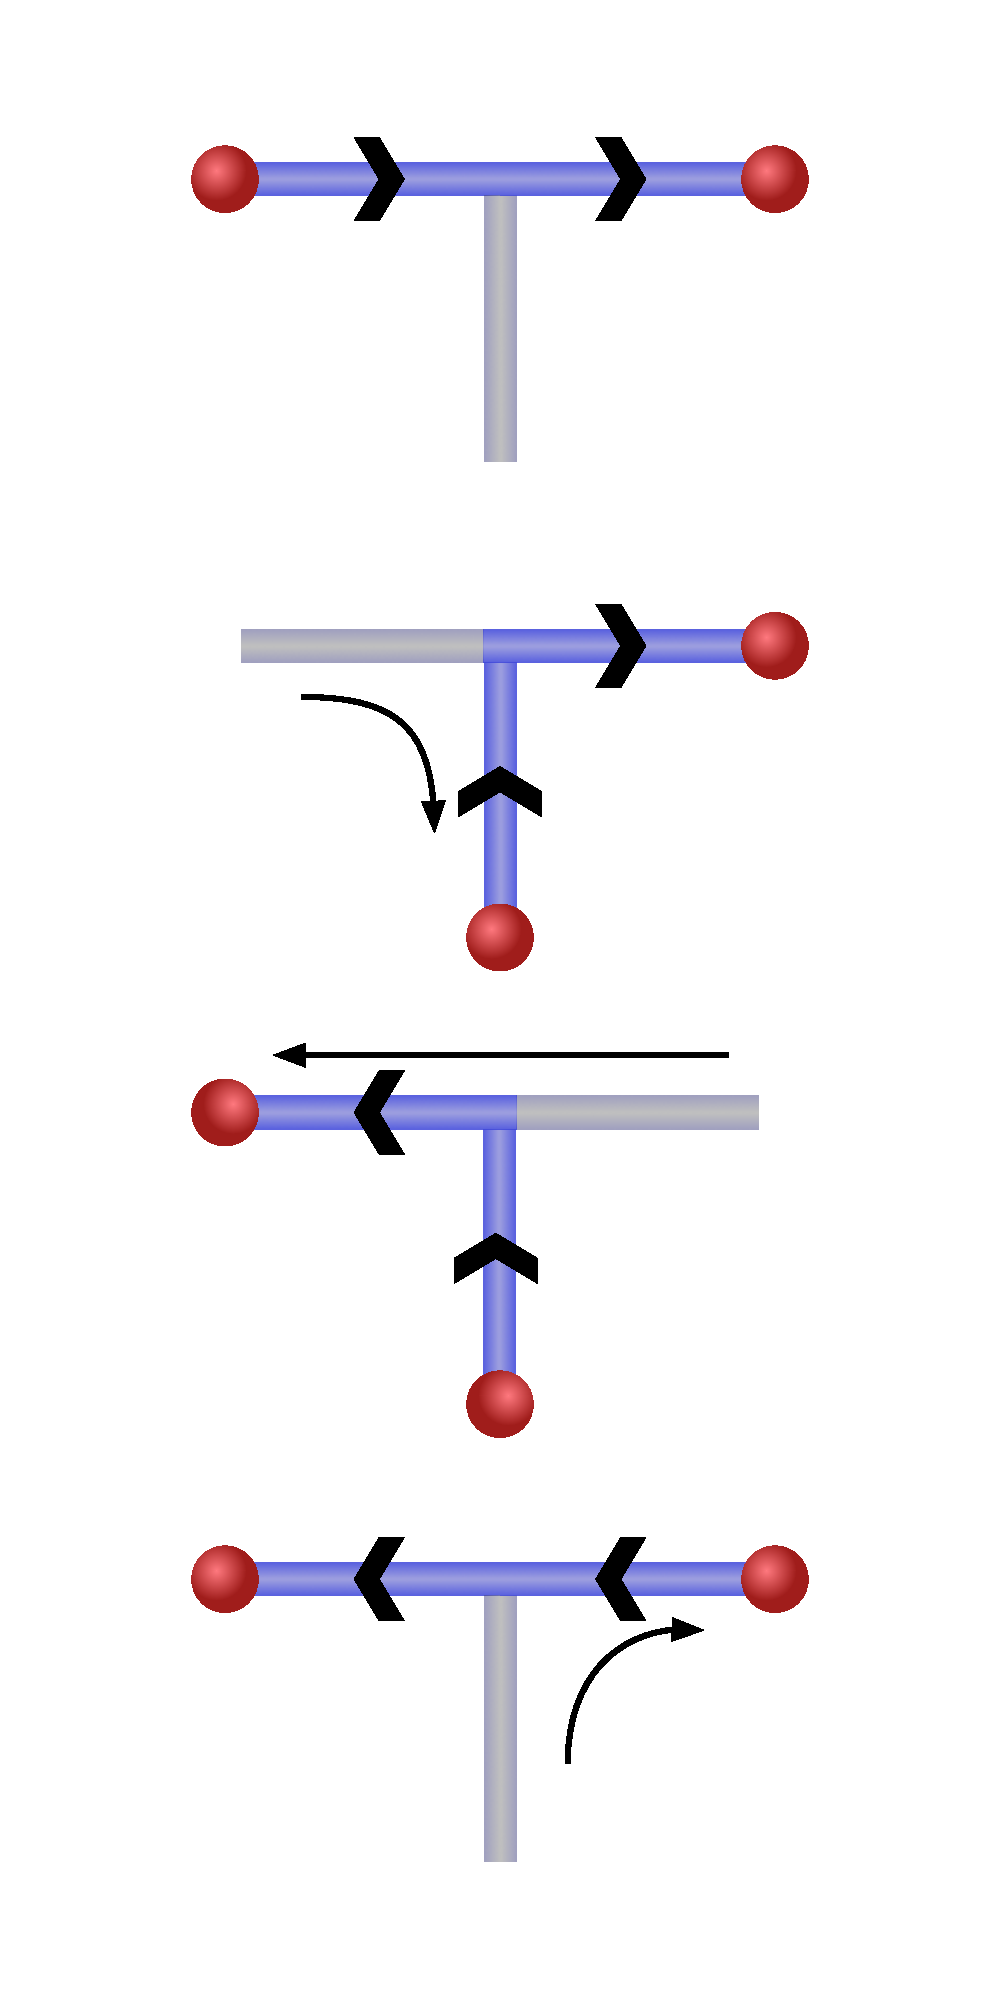
\includegraphics[width=0.25\textwidth]{../../images/t-junction.pdf}};
        \node[inner sep=0pt] (reference) at (0,-3.2) {\small Alicea, \textit{Nature Phys.} \textbf{7}, 412 (2011)}
        \end{tikzpicture}
      \end{figure}
    \end{multicols}

  \end{frame}

  \begin{frame}
    \frametitle{\MO}
    \begin{multicols}{2}

    \begin{itemize}
      \item Consider triangular islands, topologically similar to T-junctions.
      \item Islands of three-fold rotational symmetry occur naturally in epitaxial growth on close-packed metal surfaces.
      \item Good platform for transition from 2D to 1D topological superconductor.
    \end{itemize}
    \newline

    \begin{figure}
      \begin{tikzpicture}
        \node[inner sep=0pt] (figure) at (0,0)
        {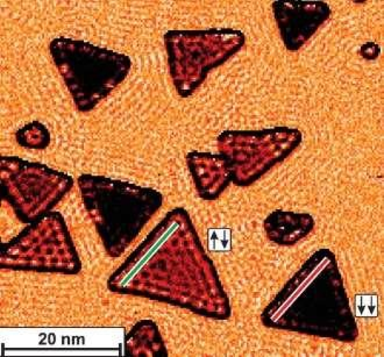
\includegraphics[width=0.4\textwidth]{../../images/triangular-islands.pdf}};
        \node[inner sep=0pt] (caption) at (0,-2.8) {\scriptsize Triangular Co islands on Cu(111).};
        \node[inner sep=0pt] (reference) at (0,-3.2) {\small Pietzsch et al., \textit{PRL} \textbf{96}, 237203 (2006)}
        \end{tikzpicture}
      \end{figure}
    \end{multicols}

  \end{frame}


  \section{\FO}

  \begin{frame}
    \frametitle{\PW}

    \begin{figure}
      \begin{tikzpicture}
        %\draw[help lines,gray!20] (-4,-4) grid[step=0.5] (4,4);
        \node[inner sep=0pt] (figure) at (-3.60,4.2)
        {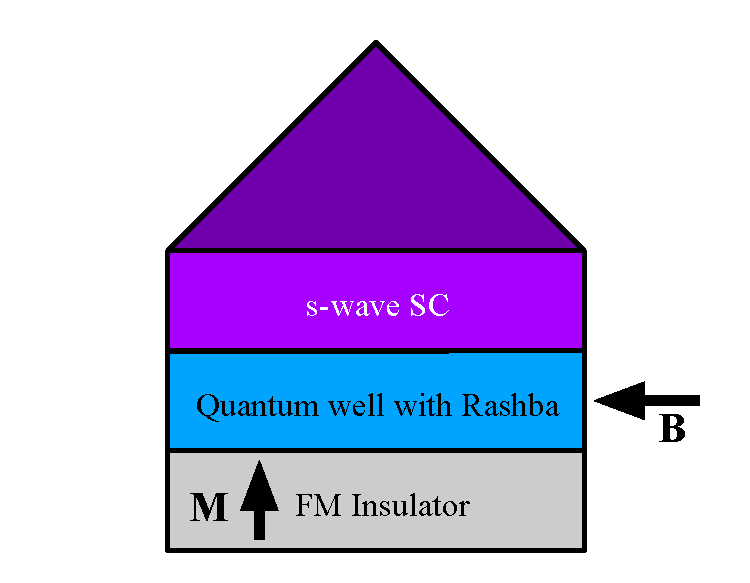
\includegraphics[width=0.35\textwidth]{../../images/tunable-semiconductor.pdf}};
        \node[inner sep=0pt] (figure) at (2.10,4.0)
        {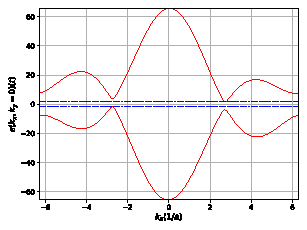
\includegraphics[width=0.40\textwidth]{../../images/dispersion-in-plane.pdf}};
        \node[inner sep=0pt] (figure) at (-3.9,0.2)
        {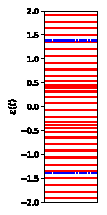
\includegraphics[width=0.14\textwidth]{../../images/energy-spectra-in-plane.pdf}};
        \node[inner sep=0pt] (figure) at (2.5,0.2)
        {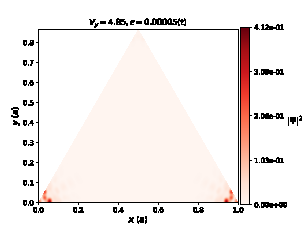
\includegraphics[width=0.40\textwidth]{../../images/wavefunction-2-in-plane.pdf}};
        %\node[inner sep=0pt,overlay] (caption) at (-6.25,3.40) {\footnotesize$V_y = 4.85$};
      \end{tikzpicture}
    \end{figure}

  \end{frame}

  \begin{frame}
    \frametitle{Kitaev Limit with Vector Potential on a Triangular Island}

    \begin{multicols}{2}
    % show condition for there to be a MF at one corner and show a picture
      \begin{tikzpicture}
        %\draw[help lines,gray!20] (-4,-4) grid[step=0.5] (4,4);
        \node[inner sep=0pt] (figure) at (0,0)
        {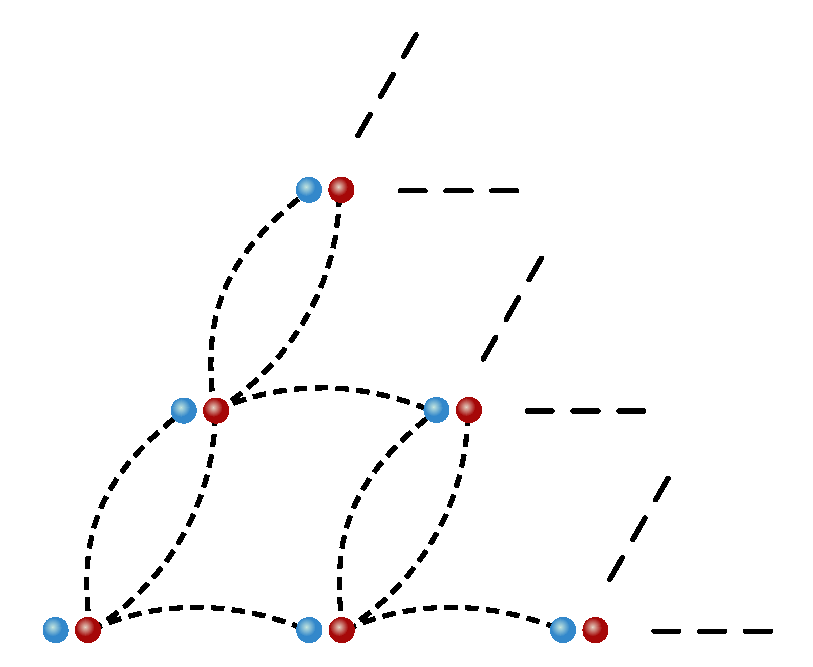
\includegraphics[width=.4\textwidth]{../../images/left-triangle-corner.pdf}};
      \end{tikzpicture}

      \small
      \begin{gather*}
        \hspace{-5em}
        \ham = \sum_{<j,l>} \left[ -t e^{i\phi_{l,j}}\cc_{l} c_j + \de e^{i\theta_{l,j}} \cc_{l}\cc_j + h.c.\right] - \sum_j \mu \cc_j c_j \\
        \hspace{-5em}
        \phi_{l,j} = -\dfrac{e}{\hbar}\int_{\vec{r}_j}^{\vec{r}_l} \vec{A} \cdot d\vec{l} \\
        \hspace{-5em}
        \vec{A} = -\dfrac{2 \pi}{3\sqrt{3} a} \hat{y}
      \end{gather*}

    \end{multicols}

  \end{frame}

  \section{\RE}

  \begin{frame}
    \frametitle{Majorana Number of 1D Chain with Vector Potential}

    % show a different kind of pairing here (phi= pi and mu = 0)

    \vspace{1em}
    \begin{tikzpicture}
      \node[inner sep=0pt] (figure) at (0,0)
      {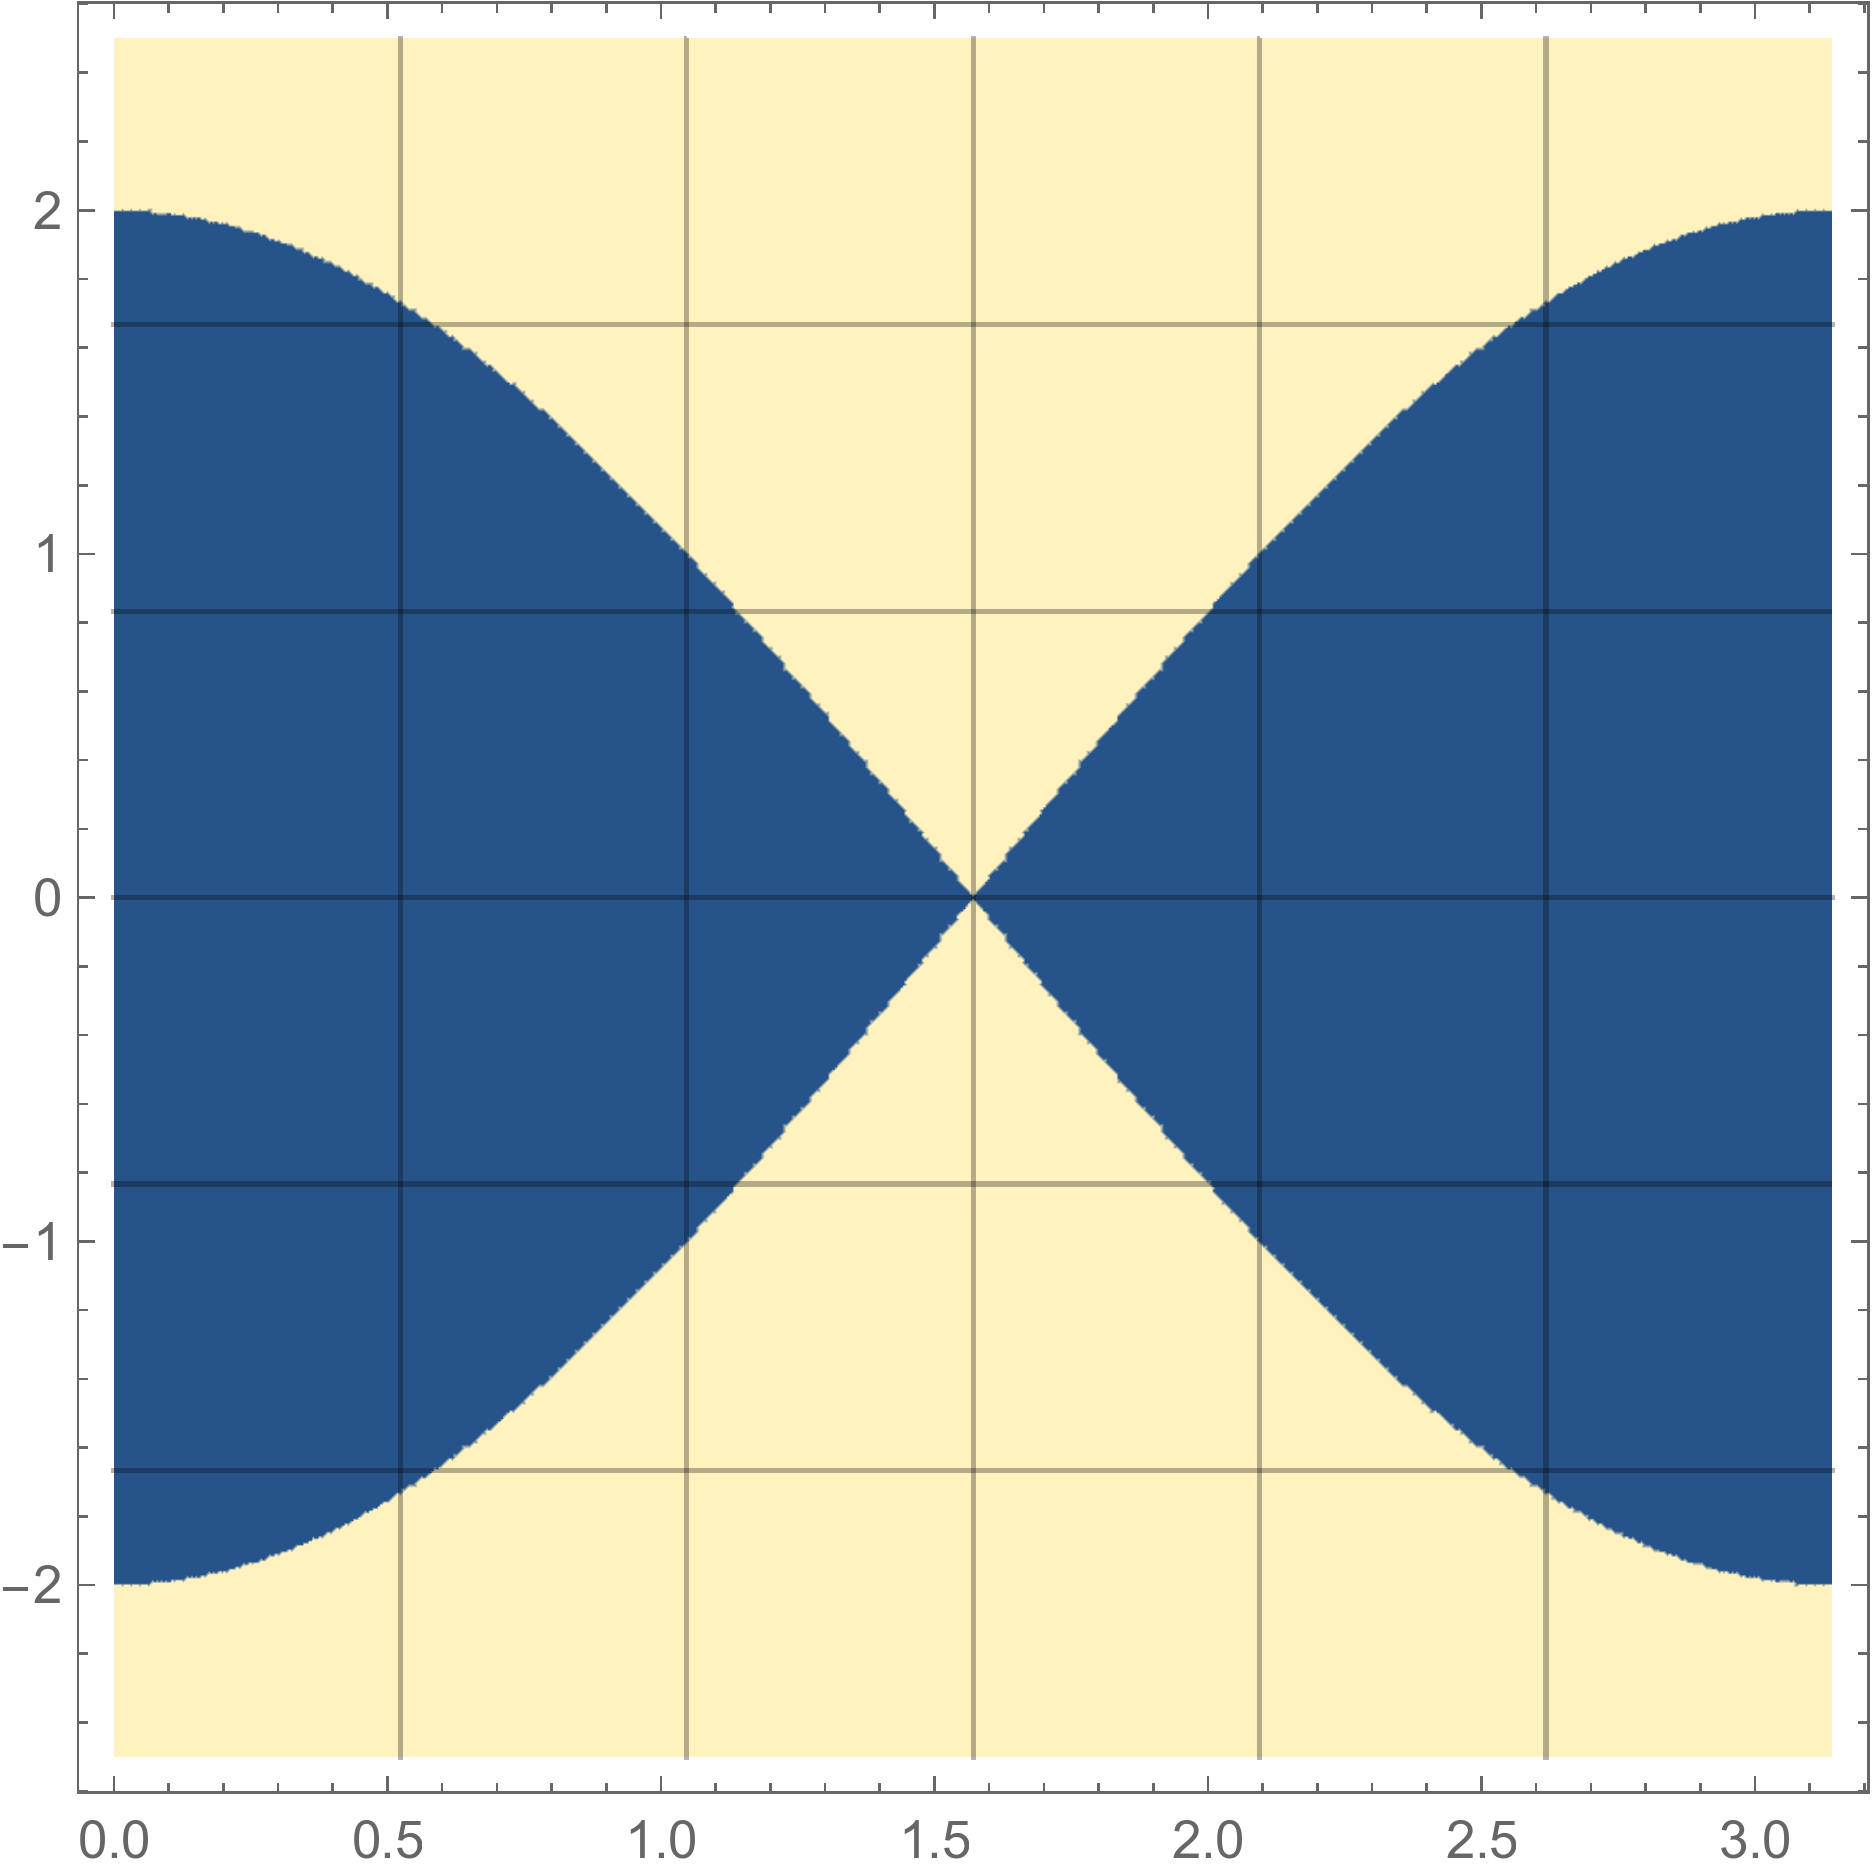
\includegraphics[width=0.4\textwidth]{../../images/Majorana-number.pdf}};
      \node[inner sep=0pt] (mu) at (-2.8,0.1) {$\mu$};
      \node[inner sep=0pt] (phi) at (0.1,-2.8) {$\phi$};
      \node[inner sep=0pt] (figure) at (0.1,-3.8)
      {\includegraphics[width=\textwidth]{../../images/kitaev-chain-mu_pi.pdf}};
      \node[inner sep=0pt] (phi0) at (-6.2,-3.825) {\footnotesize $\phi = \pi$};
    \end{tikzpicture}

  \end{frame}

  \begin{frame}
    \frametitle{Triangular Chain}
    % show spectral plot and wavefunction

    \begin{multicols}{2}
    \vspace{-2em}
    \small
    \begin{gather*}
      \vec{A}(x) = B x \hat{y} \\
      B_0 = \dfrac{8 \pi}{3\sqrt{3} a^2 (2 n_r - 3)}
    \end{gather*}

    \vspace{-4em}
    \begin{figure}
      %\hspace{-1.25em}
      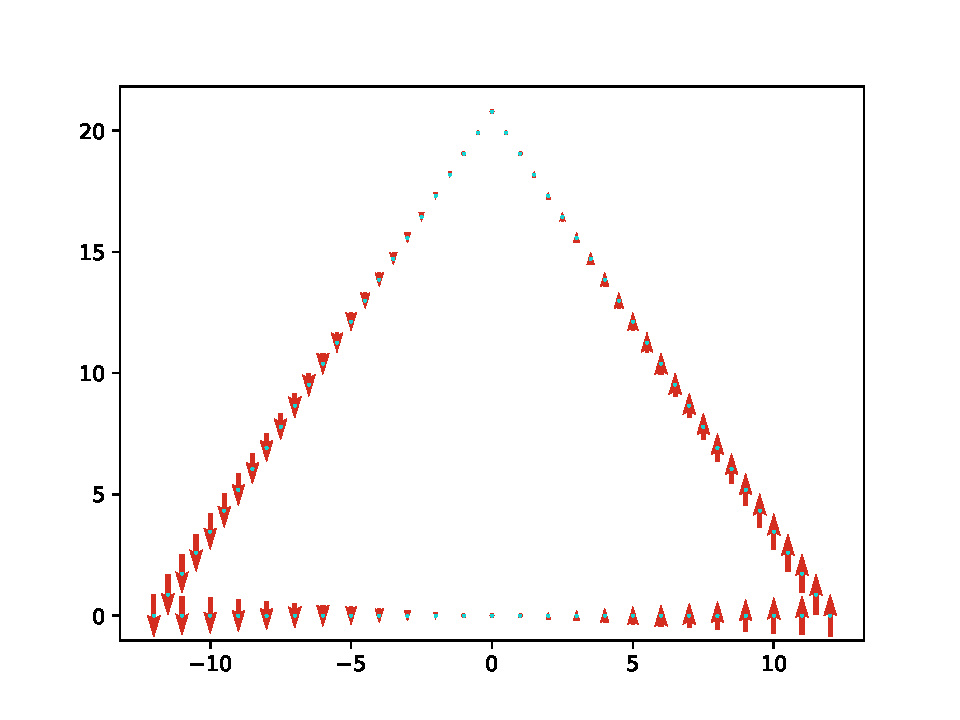
\includegraphics[width=0.4\textwidth]{../../images/vector-potential-field.pdf}
    \end{figure}

    \begin{figure}
      \center
      \hspace{-1.25em}
      \includegraphics[width=0.35\textwidth]{../../../research-code/mf-quantum-logic-gate-scripts/data/figures/linear-vector-potential/nr-25/w-1/mu-p0_0000/spectral-flow.pdf}
    \end{figure}

    \vspace{-1em}

    \begin{figure}
      \includegraphics[width=0.4\textwidth]{../../../research-code/mf-quantum-logic-gate-scripts/data/figures/linear-vector-potential/nr-25/w-1/mu-p0_0000/En01-B-0_1029.pdf}
    \end{figure}
    \end{multicols}

  \end{frame}

  \begin{frame}
    \frametitle{Hollow Triangle}

    \begin{figure}
      \begin{tikzpicture}
        \node[inner sep=0pt] (figure) at (-3.2,0)
        {\includegraphics[width=0.5\textwidth]{../../../research-code/mf-quantum-logic-gate-scripts/data/figures/linear-vector-potential/nr-25/w-3/mu-p0_0000/spectral-flow.pdf}};
        \node[inner sep=0pt] (figure) at (3.2,-0.15)
        {\includegraphics[width=0.5\textwidth]{../../../research-code/mf-quantum-logic-gate-scripts/data/figures/linear-vector-potential/nr-25/w-3/mu-p0_0000/En00-B-0_1029.pdf}};
      \end{tikzpicture}
    \end{figure}
  \end{frame}

  \section[Summary]{\CO}
  \begin{frame}
    \frametitle{\CO}

    \begin{itemize}
      \item Introduction of vector potential allows for additional tunability of topology.
      \item Triangular islands with a gapped interior can be a promising platform for hosting and manipulating MZMs.
      \item Next steps
        \begin{itemize}
          \item Search for safe MZMs in hollow triangles outside the Kitaev limit.
          \item Develop a robust braiding scheme.
        \end{itemize}
    \end{itemize}
  \end{frame}


  \appendix

  \begin{frame}
  \frametitle{Majorana fermion notation and coupling isolations}
    The complex fermion operator can be written as a superposition of two Majorana fermions $c_j = \frac{1}{2} (a_j + i b_j)$.
    Due to the nature of Majorana fermions, $a^{\dagger}_j = a_j$, the creation operator is $\cc_j = \frac{1}{2} (a_j - i b_j)$.
    \begin{align*}
      H = -\dfrac{i\mu}{4} \sum_j (a_j b_j - b_j a_j) - \dfrac{i}{4} \sum_{<j,l>} [&(t\sin\phi-\de\sin\theta) a_l a_j + (t\sin\phi+\de\sin\theta) b_l b_j \nonumber \\
      +&(t\cos\phi+\de\cos\theta) a_l b_j - (t\cos\phi-\de\cos\theta) b_l a_j].
    \end{align*}
    \begin{align}
      &(t \sin\phi_{j,l} - \de \sin\theta_{j,l}) a_l a_j, \\
      &(t \sin\phi_{j,l} + \de \sin\theta_{j,l}) b_l b_j, \\
      &(t \cos\phi_{j,l} + \de \cos\theta_{j,l}) a_l b_j, \\
      &(t \cos\phi_{j,l} - \de \cos\theta_{j,l}) b_l a_j
    \end{align}
  \end{frame}

  \begin{frame}
    \frametitle{Triangular chain degeneracy}

    \begin{figure}
      \includegraphics[width=0.8\textwidth]{../../../research-code/mf-quantum-logic-gate-scripts/data/figures/linear-vector-potential/nr-25/w-1/mu-p0_0000/En00-B-0_1029.pdf}
    \end{figure}

  \end{frame}

  \begin{frame}
    \frametitle{Hollow triangle degeneracy?}

    \begin{figure}
      \includegraphics[width=0.8\textwidth]{../../../research-code/mf-quantum-logic-gate-scripts/data/figures/linear-vector-potential/nr-25/w-3/mu-p0_0000/En01-B-0_1029.pdf}
    \end{figure}

  \end{frame}


\end{document}


